\documentclass[10pt]{beamer}
% This is done so that both 16/9 (160mm by 90mm)and
% 4/3 (128mm by 96mm) have same height 16/9*96 = 170.667
\geometry{paperwidth=170.667mm, paperheight=96mm}
\usefonttheme{serif}
%=================================================
% theme and color
%=================================================
\usetheme{Warsaw} %Themes
\definecolor{colorA}{RGB}{21, 69, 113}
\definecolor{colorB}{RGB}{140, 151, 154}
\setbeamercolor{structure}{fg=colorA,bg=colorB}
\setbeamertemplate{navigation symbols}{}
\setbeamertemplate{page number in head/foot}{}

%=================================================
% packages and new commands
%=================================================
\usepackage[ruled, linesnumbered, vlined]{algorithm2e}
\usepackage{epsfig, subfigure, amssymb, multirow, algorithmic, amsmath}
\newcommand*{\superscript}[1]{\ensuremath{^{\rm #1}}}
\newcommand*{\subscript}[1]{\ensuremath{_{\rm #1}}}
\usepackage{animate}
\usepackage{graphicx}
\usepackage[shortlabels]{enumitem}



\title[{\sc 300 Years to 300 min } \hspace{0.8cm} \insertframenumber/\inserttotalframenumber]{{\sc Run-time from 300 years to 300 min: Lessons learned in large-scale modeling in FEniCS.}}
\author[FENICS 2021 --- {\sc March 23\superscript{rd}, 2021}]{{Abhinav Gupta}, U Meenu Krishnan, Rajib Chowdhury, Anupam Chakrabarti}
\date{23 March 2021}
\institute{Department of Civil Engineering \\ Indian Institute of Technology Roorkee, India}

\begin{document}
  %------------------------------------------------
  % title page
  %------------------------------------------------
  \begin{frame}
    \begin{center}
      \vspace{0.1cm}
      
\includegraphics[height=2.4cm]{logo.pdf}
    \end{center}
    \titlepage
  \end{frame}
  %------------------------------------------------
  % your slides:
  %------------------------------------------------
  \label{intro}
\begin{frame}\frametitle{Motivation}
\centering
    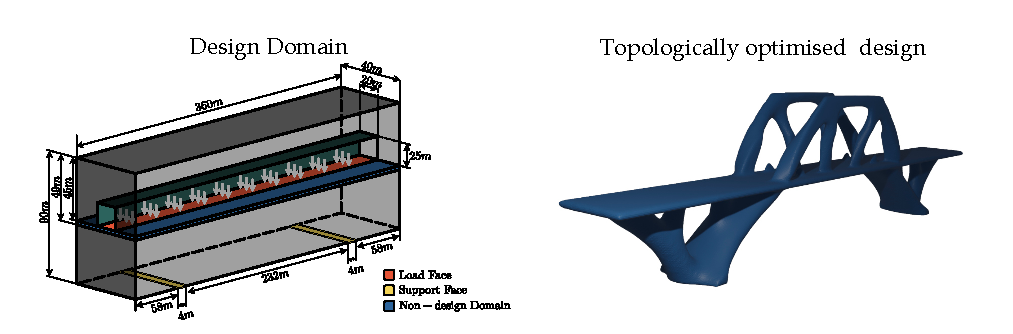
\includegraphics[width = 148mm]{slides/images/1.pdf}
    \begin{enumerate} [(I)]
        \item Solve the topology optimization problem for a medium to large scale engineering structure.
        \item The problem could contain degrees of freedom ranging from a million to over a billion.
  \end{enumerate}
\end{frame}

  %------------------------------------------------
  % example slides:
  %------------------------------------------------
  %\section{Lists}
% --------------------------------------------------- Slide --
%\subsection{Itemize}
\label{itemize}
\begin{frame}\frametitle{Lists - Itemize}
  \begin{itemize}
    \item Point A
    \item Point B
    \begin{itemize}
      \item part 1
      \item part 2
    \end{itemize}
    \item Point C
    \item Point D
  \end{itemize}
\end{frame}

% % --------------------------------------------------- Slide --
% %\subsection{Pause}
% \label{pause}
% \begin{frame}\frametitle{Lists - Itemize with Pause}
%   \begin{itemize}
%     \pause \item Point A
%     \pause \item Point B
%     \begin{itemize}
%       \pause \item part 1
%       \pause \item part 2
%     \end{itemize}
%     \pause \item Point C
%     \pause \item Point D
%   \end{itemize}
% \end{frame}

% % --------------------------------------------------- Slide --
% %\subsection{Enumerate}
% \label{enumerate}
% \begin{frame}\frametitle{Lists - Enumerate}
%   \begin{enumerate}
%     \item Point A
%     \item Point B
%     \begin{enumerate}
%       \item part 1
%       \item part 2
%     \end{enumerate}
%     \item Point C
%     \item Point D
%   \end{enumerate}
% \end{frame}

% % --------------------------------------------------- Slide --
% %\subsection{Enumerate (Roman Numerals)}
% \label{enumerateRomanNumerals}
% \begin{frame}\frametitle{Lists - Enumerate (Roman Numerals)}
%   \begin{enumerate} [(I)]
% 	\item Point A
% 	\item Point B
% 	\begin{enumerate} [(i)]
% 	  \item part 1
%       \item part 2
% 	\end{enumerate}
% 	\item Point C
% 	\item Point D
%   \end{enumerate}
% \end{frame}

  %\section{Columns}
% --------------------------------------------------- Slide --
%\subsection{Columns}
\label{columns}
\begin{frame}\frametitle{Columns}
  \begin{columns}
    \column{0.5\textwidth}
      Lorem ipsum dolor sit amet, consectetur adipisicing elit, sed do eiusmod tempor incididunt ut labore et dolore magna aliqua.
    \column{0.5\textwidth}
      Lorem ipsum dolor sit amet, consectetur adipisicing elit, sed do eiusmod tempor incididunt ut labore et dolore magna aliqua.
  \end{columns}
\end{frame}
  %\section{Figures}
% --------------------------------------------------- Slide --
%\subsection{Figures}
% \label{figures}
% \begin{frame}\frametitle{Domination on a Chessboard}
%   \begin{figure}[htb]
%     \centering
%     \begin{tabular}{cc}\pause{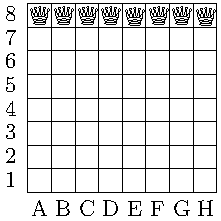
\includegraphics[scale=1]{examples/DomChess8.pdf}}&
%       \pause{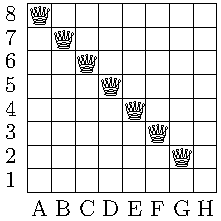
\includegraphics[scale=1]{examples/DomChess7.pdf}}\\
%       \pause{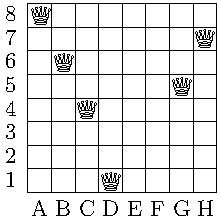
\includegraphics[scale=1]{examples/DomChess6.pdf}}&
%       \pause{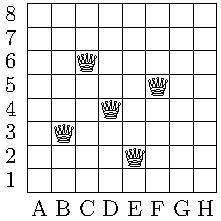
\includegraphics[scale=1]{examples/Chess1.pdf}}
%     \end{tabular}
%   \end{figure}
% \end{frame}

% --------------------------------------------------- Slide --
%\subsection{Figures}
\label{figures2}
\begin{frame}\frametitle{Single figure with caption}
  \begin{figure}[htb]
    \centering
    
\includegraphics[scale=0.25]{examples/figures/400x400.png}
    \caption{This is an caption!}
  \end{figure}
\end{frame}

  %\section{Description}
% --------------------------------------------------- Slide --
%\subsection{Description}
\label{description}
\begin{frame}\frametitle{Description Environment}
  \begin{description}
    \item[API] Application Programming Interface
    \item[LAN] Local Area Network
    \item[ASCII] American Standard Code for Information Interchange
  \end{description}
\end{frame}
  %\section{Tables}
% --------------------------------------------------- Slide --
%\subsection{Tables}
\label{tables}
\begin{frame}\frametitle{Tables}
  \begin{table}
    \begin{tabular}{l | c | c | c | c }
      Competitor Name & Swim & Cycle & Run & Total \\
      \hline \hline
      John T & 13:04 & 24:15 & 18:34 & 55:53 \\ 
      Norman P & 8:00 & 22:45 & 23:02 & 53:47\\
      Alex K & 14:00 & 28:00 & n/a & n/a\\
      Sarah H & 9:22 & 21:10 & 24:03 & 54:35 
    \end{tabular}
    \caption{Triathlon results}
  \end{table}
\end{frame}
  %\section{Blocks}
% --------------------------------------------------- Slide --
%\subsection{Blocks}
\label{blocks}
\begin{frame}\frametitle{Blocks}
  \begin{block}{Block Title}
    Lorem ipsum dolor sit amet, consectetur adipisicing elit, sed do eiusmod tempor incididunt ut labore et dolore magna aliqua.
  \end{block}
  \begin{alertblock}{Alert Block Title}
    Lorem ipsum dolor sit amet, consectetur adipisicing elit, sed do eiusmod tempor incididunt ut labore et dolore magna aliqua.
  \end{alertblock}
\end{frame}
  %\section{Definition}
% --------------------------------------------------- Slide --
%\subsection{Definition}
\label{definition}
\begin{frame}\frametitle{Definition}
  Then there’s the definition environment which produces a standard ColorA color block but with the title already specified as ‘definition’.
  \begin{semiverbatim}
    \\begin\{definition\}\newline
    A prime number is a number that...\newline
    \\end\{definition\}
  \end{semiverbatim}
  \begin{definition}
    A prime number is a number that...
  \end{definition}
\end{frame}
  %\section{Example}
% --------------------------------------------------- Slide --
%\subsection{Example}
\label{example}
\begin{frame}\frametitle{Example}
  Next there’s the example environment which produces a green block with the title ‘Example’.
  \begin{semiverbatim}
    \\begin\{example\}\newline
    Lorem ipsum dolor sit amet...\newline
    \\end\{example\}
  \end{semiverbatim}
  \begin{example}
    Lorem ipsum dolor sit amet, consectetur adipisicing elit, sed do eiusmod tempor incididunt ut labore et dolore magna aliqua.
  \end{example} 
\end{frame}
  %\section{Theorem}
% --------------------------------------------------- Slide --
%\subsection{Theorem Code}
\label{theoremCode}
\begin{frame}\frametitle{Theorem}
  There is also a group of blocks that are especially useful for presenting mathematics. For example the ‘theorem’ environment, the ‘corollary’ environment and the ‘proof’ environment.
  \begin{semiverbatim}
    \\begin\{theorem\}[Pythagoras] \newline
      $ a^2 + b^2 = c^2$ \newline
    \\end\{theorem\} \newline
    \\begin\{corollary\} \newline
      $ x + y = y + x  $ \newline
    \\end\{corollary\} \newline
    \\begin\{proof\} \newline
      $\omega +\phi = \epsilon $ \newline
    \\end\{proof\}
  \end{semiverbatim}
\end{frame}

% --------------------------------------------------- Slide --
%\subsection{Theorem Blocks}
\label{theoremBlocks}
\begin{frame}\frametitle{Theorem Blocks}
  \begin{theorem}[Pythagoras] 
    $ a^2 + b^2 = c^2$
  \end{theorem}
  \begin{corollary}
    $ x + y = y + x  $
  \end{corollary}
  \begin{proof}
    $\omega +\phi = \epsilon $
  \end{proof}
\end{frame}
  %\section{Hyperlinks}
% --------------------------------------------------- Slide --
%\subsection{Hyperlinks Code}
\label{hyperlinks}
\begin{frame}\frametitle{Hyperlink}
Before we can create any hyperlinks we need to tag the frames we want to link to using the \label command.
 
\hyperlink{contents}{click here}
\hyperlink{section1}{\beamerbutton{section 1 page}}
\hyperlink{columns}{\beamergotobutton{columns page}}
\hyperlink{pictures}{\beamerskipbutton{pictures page}}
\hyperlink{pictures}{\beamerreturnbutton{pictures page}}

\end{frame}
  \SetKwInOut{Input}{Input}\SetKwInOut{Output}{Output}
\begin{frame}\frametitle{A trivial Set Cover algorithm}
\begin{algorithm}[H]\footnotesize
        \Input{A set cover instance $({\cal S,U})$ and a variable ${\cal S}_{\rm dom}$.}
        \Output{A minimum set cover of $({\cal S,U})$.}
\If{${\cal S}=\emptyset$}{
\Return $\emptyset$\;
}
Let $S \in {\cal{S}}$ be a set of maximum cardinality\;
${\cal{C}}_1 = \{S\}\cup {\tt MSC}(\{S'\backslash S \mid S' \in{\cal S}\backslash \{S\}\}, {\cal U}\backslash S )$\;
${\cal{C}}_2 = {\tt MSC}({\cal S}\backslash \{S\},{\cal U})$\;
${\cal S}_{\rm dom} \leftarrow \emptyset$\;
\If{${\cal U} \subseteq {\cal C}_1$}{
${\cal S}_{\rm dom} \leftarrow {\cal C}_1$\;
\If{${\cal U} \subseteq {\cal C}_2$}{
\If{$|{\cal C}_2| < |{\cal C}_1|$}{
${\cal S}_{\rm dom} \leftarrow {\cal C}_2$\;
}
}
}
\Return ${\cal S}_{\rm dom}$\;
\caption{{\tt MSC}$({\cal S,U})$}
\end{algorithm}
\end{frame}
  %------------------------------------------------
  % End
  %------------------------------------------------
  \label{conclusion}
\begin{frame}\frametitle{Conclusion}
  \begin{enumerate} [(I)]
	\item General guidelines for handling medium to large-scale systems in FEniCS
	\begin{enumerate} [(i)]
      \item Always profile the code and look for bottlenecks.
      \item Avoid use of loops in python. Look for efficient alternatives.
      \item Avoid re-evaluation of matrices that do not change.
      \item Evaluate and write only necessary simulation outputs.
      \item In an iterative process evaluate output at every $n^{th}$ step to further speed up the simulation.
	  \item Properly select/configure the solver and preconditioner based on the problem.

	\end{enumerate}
	\item Stepping into the realm of large scale simulations require knowledge of good programming practices, parallelization, and a deep understanding of the working principles of the tools/libraries.
  \end{enumerate}
\end{frame}

  \begin{frame}
\centering
Thanks

\rule{180pt}{1pt}

iitrabhi@gmail.com

computationalmechanics.in
\end{frame}

  %%%%%%%%%%%%%%%%%%
%
% bibliography
%
%%%%%%%%%%%%%%%%%%

\begin{frame} \frametitle{References}
\begin{thebibliography}{xx}\footnotesize
	\bibitem[1]{Hughes}
		Hughes, T. J.R. and Cottrell, J. A. and Bazilevs, Y., 
		Isogeometric analysis: CAD, finite elements, NURBS, exact geometry and mesh refinement, 
		\textit{Computer Methods in Applied Mechanics and Engineering}, 194(39–-41),  4135--4195, 2005.
		
	\bibitem[2]{Kiendl}
		Kiendl,J. ,Bletzinger,K.-U., Linhard,J., Wüchner, R.,
		Isogeometric shell analysis with Kirchhoff–Love elements, 
		\textit{Computer Methods in Applied Mechanics and Engineering}, 198(49-52), 3902--3914, 2009.
		
	\bibitem[3]{Nguyen}
		Nguyen, V. P., Anitescu, C., Bordas, S. P. A.,and Rabczuk, T. , 
		Isogeometric analysis: An overview and computer implementation aspects, 
		\textit{Mathematics and Computers in Simulation}, 117, 89--116, 2015.

	\bibitem[4]{Zareh}
		Zareh, M.,and Qian, X. , 
		Kirchhoff–Love shell formulation based on triangular isogeometric analysis, 
		\textit{Computer Methods in Applied Mechanics and Engineering}, 347, 853--873, 2019.

	\bibitem[5]{Bletzinger}
		Bletzinger, K. U.,and Ramm, E., 
		Form finding of shells by structural optimization, 
		\textit{Engineering with Computers}, 9(1), 27--35, 1993.

	\bibitem[6]{Bandara}
		Bandara, K., and Cirak, F. , 
		Isogeometric shape optimisation of shell structures using multiresolution subdivision surfaces, 
		\textit{CAD Computer Aided Design}, 95, 62--71, 2018.

	\bibitem[7]{Hirschler}
		Hirschler, T., Bouclier, R., Duval, A., Elguedj, T.,and Morlier, J.,
		Isogeometric sizing and shape optimization of thin structures with a solid-shell approach, 
		\textit{Structural and Multidisciplinary Optimization}, 2018.
\end{thebibliography}
\end{frame}
\end{document}
